Consideremos una red bidimensional cuadrada, donde cada uno de los casilleros puede estar o no ocupado, formando un patrón.
De acuerdo a la geometría integral, existen tres funcionales aditivas (las funcionales de Minkowski) que describen el contenido morfológico de dicho patrón: el área $A$, el perímetro $U$ y la característica de Euler $\chi$, que describe la topología del patrón: en dos dimensiones, $\chi$ es el número de regiones de casilleros ocupados que están completamente conectados menos el número de regiones completamente conectadas por casilleros vacíos. Decimos que dos casilleros están ``conectados'' si y sólo si son primeros o segundos vecinos o pueden ser conectados a través de casilleros ocupados que son primeros o segundos vecinos.

Conceptualmente, el procedimiento para calcular estas funcionales consta de dos partes. Primero, descomponemos cada casillero en 4 vértices, 4 lados y el interior del casillero, como en la figura~\ref{fig:mink_2d}. Luego contamos la cantidad de interiores de casilleros $n_s$, lados $n_e$ y vértices $n_v$ y calculamos el área $A$, perímetro $U$ y característica de Euler $\chi$ mediante:
\begin{equation}
A = n_s, \qquad U = -4\,n_s + 2\,n_e \qquad \chi = n_s - n_e + n_v
\end{equation}
Para el ejemplo de la figura~\ref{fig:mink_2d} hallamos $A = 8$, $U = 16$ y $\chi = 0$.

\begin{figure}[h] %figure 3
\centering
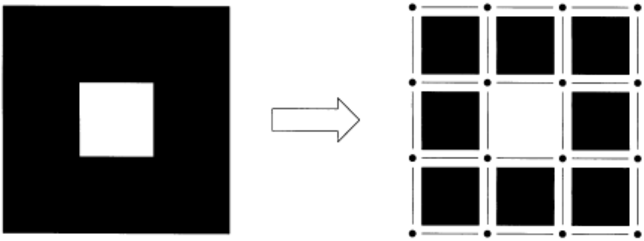
\includegraphics[width=0.7\columnwidth]{minkowski/mink_2d}
\caption{Ejemplo de implementación de la digitalización y cálculo de funcionales de Minkowski en dos dimensiones, extraída de~\cite{michielsen_integral-geometry_2001}.}
\label{fig:mink_2d}
\end{figure}


Para una red cúbica tridimensional, hay 4 funcionales de Minkowski: el volumen $V$, la superficie $S$, el ancho medio $B$ y la característica de Euler $\chi$.
Así como en el caso bidimensional, el primer paso para calcular estos tres números es considerar cada casillero como la unión de 8 vértices, 12 lados, 6 caras y el interior del cubo.
A partir de esto, análogamente con el caso 2D, las funcionales de Minkowski se pueden calcular como:
\begin{equation}
V = n_c, \qquad S = -6\,n_c + 2\,n_f \qquad 2\,B = 3\,n_c - 2\,n_f + n_e \qquad \chi = -n_c + n_f - n_e + n_v
\end{equation}
donde $n_c$ es el número de casilleros y $n_f$ el número de caras.

El procedimiento entonces para encontrar estas funcionales de Minkowski para las estructuras que se forman es entonces el de digitalizar la estructura: a cada partícula le asignamos un radio $r_p$ y subdividimos el espacio tridimensional en una grilla cúbica.
Decimos que un sitio de esa grilla está ocupado sí existe al menos una partícula a distancia $d<r_p$ de dicho sitio.
Una vez que tenemos la estructura \emph{digitalizada}, procedemos a contar cubos, caras, vértices y lados para encontrar las funcionales de Minkowski.